\chapter{Ecuaciones de movimiento y análisis de vibraciones}
\label{ch:operacion}
\section{Movimiento impuesto y coordenadas desconocidas}
La función $\psi(t)=\psi_0+\Omega t$ describe una operación prescrita: su evolución se proporciona al modelo y no se obtiene resolviendo una ecuación de balance para el accionamiento. El par necesario para mantenerla puede ser una reacción del sistema idealizado. Por consiguiente, no se supone que el rotor gire libremente con momento angular constante. Velocidad angular impuesta y momento angular conservado son condiciones físicas distintas.

Una vez fijado ese movimiento, las coordenadas estructurales independientes se reúnen en $\vct q$. Incluyen desplazamientos y rotaciones de perturbación compatibles con los vínculos, mientras que $\psi$ es un dato. En la representación con conexión elástica se prescribe la rotación nominal del accionamiento y se conserva la torsión relativa del cubo como incógnita. Su ángulo total puede diferir de $\psi$ por una pequeña perturbación, determinada por la rigidez de la conexión y por las acciones del sistema. El caso de velocidad instantánea del cubo impuesta exactamente se obtiene restringiendo esa coordenada relativa.

En lo que sigue se estudia primero un estado estacionario relativo, para el cual los coeficientes expresados en las coordenadas elegidas no dependen explícitamente del tiempo. Esta hipótesis no se deduce solamente de $\Omega=\mathrm{constante}$. La gravedad sobre una pala giratoria, la interacción con una torre no giratoria o una carga no uniforme pueden producir coeficientes o fuerzas periódicos. El caso periódico se distingue al final del capítulo.

\section{Descomposición de la energía cinética}
\subsection{Grado en las velocidades generalizadas}
La cinemática de un sistema con movimiento impuesto permite que una partícula tenga velocidad distinta de cero aun cuando $\dot{\vct q}=\vct0$. Por ello, la energía cinética no es necesariamente una forma puramente cuadrática homogénea en $\dot{\vct q}$. Siguiendo la descomposición de sistemas no naturales expuesta por Meirovitch \cite[sección 4.1]{meirovitch}, se escribe
\begin{align}
 T(\vct q,\dot{\vct q})&=T_2+T_1+T_0,\\
 T_2&=\tfrac12\dot{\vct q}^{\tr}\mathsf M(\vct q)\dot{\vct q},\\
 T_1&=\dot{\vct q}^{\tr}\vct a(\vct q),\qquad
 T_0=T(\vct q,\vct0;\Omega).
 \label{eq:Tdecomp}
\end{align}
El subíndice indica el grado respecto de las velocidades generalizadas: dos, uno o cero. No indica el orden de una expansión en amplitud de desplazamiento. En particular, $T_0$ puede depender de $\vct q$ y no es una constante simplemente por llevar subíndice cero. El vector $\vct a$ de esta sección es el coeficiente de $T_1$, no la aceleración de una partícula; su argumento aclara el uso local del símbolo.

Si $V(\vct q)$ contiene las contribuciones con potencial de posición, se define el potencial efectivo o dinámico
\begin{equation}
 U_{\rm eff}(\vct q)=V(\vct q)-T_0(\vct q).
 \label{eq:Ueff}
\end{equation}
La función $T_0$ sigue siendo parte de la energía cinética física. Su signo negativo en $U_{\rm eff}$ procede de reorganizar el lagrangiano $L=T-V$ después de prescribir el movimiento, y no de convertir toda la dinámica en un problema conservativo. El accionamiento puede intercambiar energía con la estructura; las cargas aerodinámicas y la disipación se introducen por separado.

\subsection{Contribución nominal de una distribución de masa}
Considérese un cuerpo rígido, o una sección por unidad de longitud, en un sistema de referencia cuyo eje gira uniformemente. Sea $\vct y_C$ la posición de su centro de masa respecto al origen del eje y $Q$ su orientación relativa a ese sistema de referencia. Todas las componentes de esta subsección se expresan en él. Para un cuerpo de masa $m$ e inercia centroidal $J_C$ expresada en la base corporal,
\begin{equation}
 T_0=\tfrac12m\|W\vct y_C\|^2
 +\tfrac12\vct\Omega^{\tr}QJ_CQ^{\tr}\vct\Omega,
 \qquad W=[\vct\Omega]_\times.
 \label{eq:T0rigid}
\end{equation}
El primer término corresponde al desplazamiento orbital del centro de masa; el segundo, a la rotación de la distribución alrededor de su centro. Para una sección se sustituyen $m,J_C$ por $\mu,j_C$ y se integra sobre la longitud. El centro $\vct y_C$ incluye el brazo de conexión de la raíz, la posición longitudinal y la excentricidad de masa. Omitir el término orbital pierde gran parte de la contribución nominal de una pala al rotor.

El potencial asociado a esta contribución cinemática se puede escribir $V_\Omega=-T_0$. Para una masa puntual en $\vct y$,
\begin{equation}
 V_\Omega=-\tfrac12m\|W\vct y\|^2,
 \qquad -\frac{\partial V_\Omega}{\partial\vct y}
 =-mW^2\vct y.
\end{equation}
Este último vector es la carga inercial equivalente que aparece al formular el balance en el sistema de referencia giratorio. En cambio, la aceleración absoluta del punto fijo en ese sistema de referencia es $W^2\vct y$, dirigida hacia el eje. Son términos de signos opuestos ubicados en lados distintos del balance. El hecho de que la aceleración centrípeta cambie de dirección durante el giro no basta para clasificarla como una fuerza no conservativa. La existencia de $V_\Omega$ aquí depende de la velocidad de giro prescrita constante y de la descripción adoptada; no debe extenderse sin derivación a movimientos impuestos arbitrarios.

En una pala deformable, el giro puede generar esfuerzo axial y modificar la rigidez tangente. La contribución geométrica debida a ese esfuerzo y la derivada de $-T_0$ deben obtenerse a partir del mismo balance de equilibrio. Sumar una rigidez de pretensión aproximada a un hessiano que ya contiene el mismo efecto produce doble contabilización.

\section{Equilibrio relativo y movimiento sincrónico}
Un estado $\vct q_0$ constante en coordenadas apropiadas satisface
\begin{equation}
 \nabla U_{\rm eff}(\vct q_0)=\vct Q_0,
 \qquad \vct Q_0=\vct Q_{\rm nc}(\vct q_0,\vct0),
 \label{eq:equilibrio}
\end{equation}
donde $\vct Q_{\rm nc}$ reúne cargas generalizadas que no se han incluido en $V$. Esta igualdad caracteriza un equilibrio relativo, no el reposo absoluto de todas las partículas. Las partículas del rotor continúan describiendo el movimiento nominal y poseen velocidad y aceleración. La deformación que permanece fija en el sistema de referencia del rotor se transporta sincrónicamente con él.

Conviene separar tres objetos: la geometría material de referencia $\mathcal B_0$, la trayectoria nominal prescrita y el estado de operación deformado $\vct q_0$. El último depende de $\Omega$, cargas, rigideces y restricciones. No es necesariamente cero ni coincide con la geometría descargada. Una perturbación $\vct\eta(t)$ produce
\begin{equation}
 \vct q(t)=\vct q_0+\vct\eta(t).
\end{equation}
El estado de operación es la base de la linealización; las vibraciones se describen mediante $\vct\eta$. La palabra sincrónico se utiliza aquí para el transporte de la configuración relativa con el giro nominal. No implica que cualquier frecuencia propia sea igual a $\Omega$.

\subsection{Ejemplo elemental de equilibrio en un sistema de referencia giratorio}
Una masa $m$ se desplaza radialmente en una guía que gira a velocidad impuesta $\Omega$ y se une al eje mediante un resorte de rigidez $k$ y longitud natural $\ell$. Su coordenada radial es $r$. El ejemplo no representa una pala: permite distinguir movimiento y perturbación sin introducir matrices. Se tiene
\begin{equation}
 T=\tfrac12m\dot r^2+\tfrac12m\Omega^2r^2,
 \quad V=\tfrac12k(r-\ell)^2,
 \quad U_{\rm eff}=\tfrac12k(r-\ell)^2-\tfrac12m\Omega^2r^2.
\end{equation}
La ecuación radial y el equilibrio, cuando $k>m\Omega^2$, son
\begin{equation}
 m\ddot r+(k-m\Omega^2)r=k\ell,
 \qquad r_0=\frac{k\ell}{k-m\Omega^2}.
\end{equation}
Aunque $r_0$ es constante, la masa describe una circunferencia en el sistema de referencia newtoniano. Con $r=r_0+\eta$, la perturbación cumple $m\ddot\eta+(k-m\Omega^2)\eta=0$. La reacción transversal de la guía y el accionamiento hacen posible mantener el giro impuesto. Este ejemplo ilustra el potencial efectivo y no implica que el giro reduzca todas las frecuencias de una estructura: una pala incorpora también flexión, tensiones de operación y acoplamientos ausentes aquí.

La figura~\ref{fig:guia} muestra la guía y la trayectoria circular en una vista espacial: una coordenada radial constante es compatible con la rotación prescrita del conjunto.

\begin{figure}[htbp]
\centering
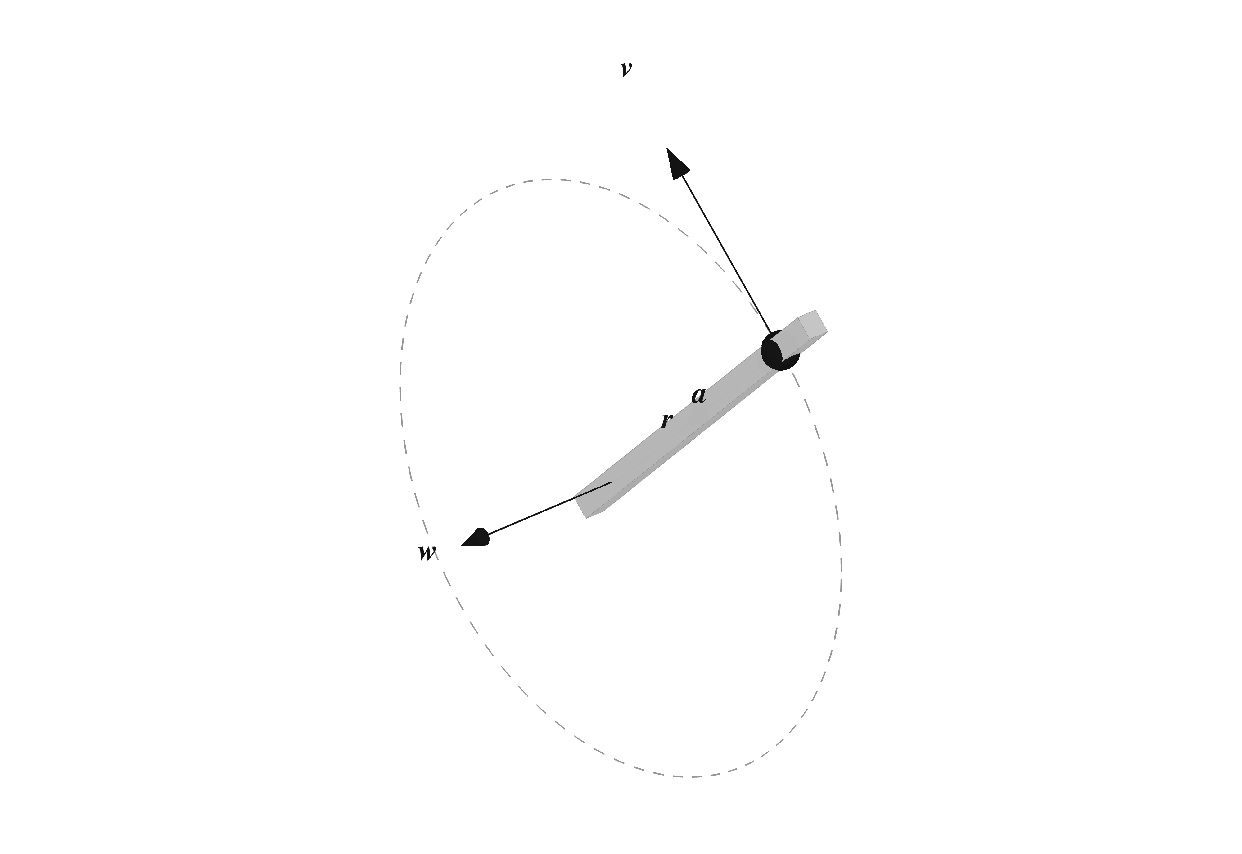
\includegraphics[width=.96\linewidth,height=.40\textheight,keepaspectratio]{figures/tecplot/concept_guia.pdf}
\caption[Equilibrio relativo en una guía giratoria]{Equilibrio relativo de un punto en una guía giratoria. La distancia radial constante es compatible con velocidad tangencial y aceleración centrípeta en el sistema inercial. La trayectoria discontinua y la guía con espesor distinguen el movimiento absoluto de la coordenada relativa.}\label{fig:guia}
\end{figure}

\section{Linealización alrededor del equilibrio de operación}
La linealización alrededor del equilibrio, presentada por Meirovitch en un paso distinto de la descomposición anterior \cite[sección 4.4]{meirovitch}, se obtiene reteniendo términos de grado total dos en el lagrangiano perturbado. Se definen
\begin{equation}
 \mathsf M_0=\mathsf M(\vct q_0),\quad
 A_{ij}=\left.\frac{\partial a_i}{\partial q_j}\right|_{\vct q_0},\quad
 \mathsf K_U=\left.\nabla^2 U_{\rm eff}\right|_{\vct q_0}.
\end{equation}
El término $\dot{\vct\eta}^{\tr}\vct a(\vct q_0)$ es una derivada temporal total si $\vct a(\vct q_0)$ es constante, y no altera las ecuaciones. Una vez balanceados los términos lineales por el equilibrio, la parte relevante de segundo grado es
\begin{equation}
 L^{(2)}=\tfrac12\dot{\vct\eta}^{\tr}\mathsf M_0\dot{\vct\eta}
 +\dot{\vct\eta}^{\tr}A\vct\eta
 -\tfrac12\vct\eta^{\tr}\mathsf K_U\vct\eta.
\end{equation}
El producto de la variación de $\mathsf M$ con dos velocidades perturbadas sería de tercer grado; por ello se evalúa la masa en $\vct q_0$. Aplicando las ecuaciones de Lagrange a la parte conservativa se obtiene
\begin{equation}
 \mathsf M_0\ddot{\vct\eta}
 +\underbrace{(A-A^{\tr})}_{\mathsf G}\dot{\vct\eta}
 +\mathsf K_U\vct\eta=\delta\vct Q_{\rm nc}.
 \label{eq:linearG}
\end{equation}
Así aparece la matriz giroscópica $\mathsf G$, con $\mathsf G^{\tr}=-\mathsf G$. No se postula su forma únicamente a partir de un momento angular nominal. El término de velocidad realiza potencia nula:
\begin{equation}
 \dot{\vct\eta}^{\tr}\mathsf G\dot{\vct\eta}=0.
\end{equation}
Puede intercambiar energía entre componentes del movimiento sin disiparla directamente. No es un amortiguamiento viscoso positivo ni la derivada de un potencial de posición.

\section{Deducción de la matriz giroscópica de un cuerpo rígido}
\subsection{Parte traslacional y parte angular}
Se consideran pequeñas coordenadas relativas $\vct z=[\vct u^{\tr},\vct\theta^{\tr}]^{\tr}$ en un sistema de referencia que gira uniformemente, con $\vct\theta$ parametrizada por la representación exponencial. Se emplea una parametrización incremental centrada en el estado de linealización: en él $\vct z=0$, y su orientación se incorpora previamente a las propiedades. Sea $\vct c$ el vector desde el punto de referencia hasta el centro de masa, y $J$ la matriz de inercia centroidal en esa misma base. Defínanse
\begin{equation}
 B=\begin{bmatrix}\Id&-[\vct c]_\times\end{bmatrix},\qquad
 E_\theta=\begin{bmatrix}0&\Id\end{bmatrix},\qquad W=[\vct\Omega]_\times.
\end{equation}
La perturbación lineal del centro es $B\vct z$ y su velocidad relativa lineal $B\dot{\vct z}$. Al expandir la energía traslacional, el término mixto relevante es $m(B\dot{\vct z})^{\tr}W(B\vct z)$; su parte antisimétrica produce $2mB^{\tr}WB$.

La rotación requiere conservar la precisión de segundo orden: la velocidad angular relativa no puede reemplazarse por $\dot{\vct\theta}$ antes de formar todos los términos mixtos. En efecto,
\begin{equation}
 \vct\omega=\vct\Omega+\dot{\vct\theta}
 +\tfrac12[\vct\theta]_\times\dot{\vct\theta}+O(3),
 \quad QJQ^{\tr}=J+[\vct\theta]_\times J-J[\vct\theta]_\times+O(2).
\end{equation}
Aquí $O(3)$ cuenta grado total en amplitudes y velocidades perturbadas; el término nominal $\vct\Omega$ no es pequeño. Al sustituir en $\tfrac12\vct\omega^{\tr}QJQ^{\tr}\vct\omega$, los términos mixtos pueden reunirse como
\begin{equation}
 \dot{\vct\theta}^{\tr}A_\theta\vct\theta,
 \qquad A_\theta=JW-\tfrac12[J\vct\Omega]_\times.
\end{equation}
Su parte antisimétrica da
\begin{equation}
 \mathsf G_\theta=JW+WJ-[J\vct\Omega]_\times.
\end{equation}
Por tanto, la matriz completa de seis coordenadas es
\begin{equation}
 \boxed{\mathsf G_6=2mB^{\tr}WB+
 E_\theta^{\tr}\bigl(JW+WJ-[J\vct\Omega]_\times\bigr)E_\theta.}
 \label{eq:G6}
\end{equation}
Cada bloque se obtiene de la misma cinemática y de la misma elección de coordenadas. Si se usan componentes angulares corporales o se linealizan directamente ecuaciones de Euler, la forma intermedia puede cambiar; se debe transformar también la cinemática para comparar matrices. No basta con sustituir $\mathsf G_\theta$ por $-[J\vct\Omega]_\times$ conservando sin cambios las restantes definiciones.

\subsection{Caso centroidal y ejes principales}
Para $\vct c=\vct0$, $J=\diag(J_1,J_2,J_3)$ y $\vct\Omega=(\Omega,0,0)^{\tr}$,
\begin{equation}
 \mathsf G_6=\begin{bmatrix}2mW&0\\0&\mathsf G_\theta\end{bmatrix},
 \qquad
 \mathsf G_\theta=\Omega
 \begin{bmatrix}0&0&0\\0&0&-(J_2+J_3-J_1)\\0&J_2+J_3-J_1&0\end{bmatrix}.
\end{equation}
La combinación de inercias es consecuencia de la parametrización relativa empleada. La nulidad de alguna combinación en una idealización geométrica no demuestra ausencia de todos los efectos de giro: permanecen contribuciones traslacionales, excentricidades, restricciones y términos dependientes de $\Omega^2$.

Para una viga se construye la expresión seccional $\mathsf G_s$ con $\mu,j_C,\vct c_m$ y se usa la interpolación cinemática del capítulo anterior:
\begin{equation}
 \mathsf G_e=\int_0^{L_e}N^{\tr}\mathsf G_sN\,\dd S.
\end{equation}
La orientación, el ensamblaje y las restricciones se aplican después con las mismas transformaciones que para masa y rigidez. Si un cambio de coordenadas depende del tiempo, sus derivadas también generan términos de transporte, como se mostró en la reducción temporal. No se deben añadir dos veces efectos que ya están representados por esas derivadas.

La figura~\ref{fig:acoplamiento-giroscopico} representa la acción de un bloque antisimétrico de dos componentes. Si $\vct w=(\dot\theta_2,\dot\theta_3)^\tr$ y $g_\theta=(J_2+J_3-J_1)\Omega$, el bloque angular anterior produce
\begin{equation}
 \vct h_g=
 \begin{bmatrix}0&-g_\theta\\g_\theta&0\end{bmatrix}\vct w,
 \qquad \vct w^\tr\vct h_g=0.
\end{equation}
En el esquema se representan las direcciones normalizadas $\widehat{\vct w}=\vct w/\|\vct w\|$ y $\widehat{\vct h}_g=\vct h_g/\|\vct h_g\|$, para vectores no nulos. Aquí $\vct h_g$ es el término inercial generalizado de ese bloque; no se introduce una acción externa adicional. Su ortogonalidad con la velocidad explica la potencia nula y no impide que cambien los modos del sistema acoplado.

\begin{figure}[htbp]
\centering
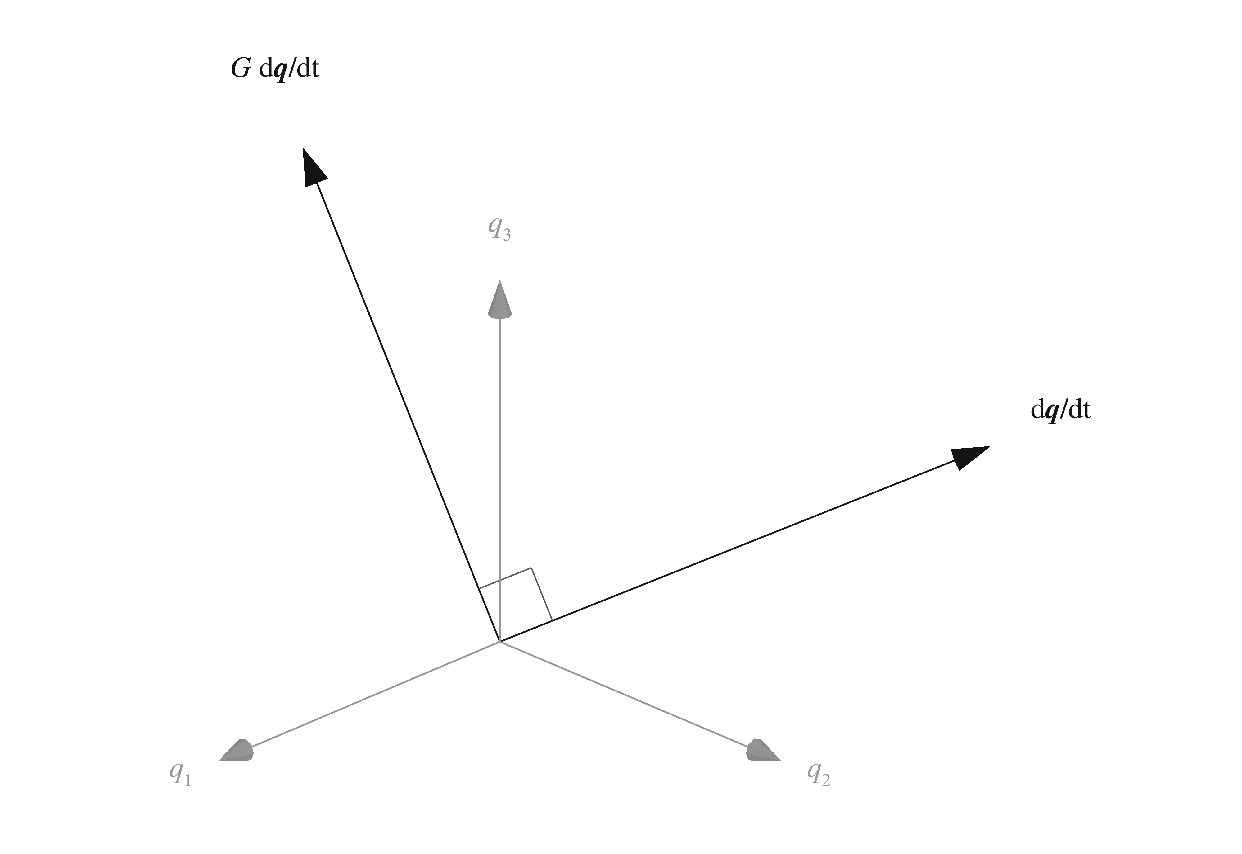
\includegraphics[width=.96\linewidth,height=.40\textheight,keepaspectratio]{figures/tecplot/concept_acoplamiento-giroscopico.pdf}
\caption[Antisimetría del acoplamiento giroscópico]{Representación geométrica de una contribución giroscópica antisimétrica. Los vectores $\dot{\vct q}$ y $G\dot{\vct q}$ son ortogonales, de modo que $\dot{\vct q}^{\tr}G\dot{\vct q}=0$. El triedro identifica coordenadas del espacio de perturbaciones; el dibujo ilustra esta identidad y no una forma modal calculada.}\label{fig:acoplamiento-giroscopico}
\end{figure}

\section{Cargas generalizadas y amortiguamiento}
Alrededor del estado de operación, una carga generalizada diferenciable puede escribirse
\begin{equation}
 \delta\vct Q_{\rm nc}=\mathsf Q_q\vct\eta+
 \mathsf Q_v\dot{\vct\eta}+\vct f(t).
\end{equation}
Con un amortiguamiento estructural separado $\mathsf C_d$, la ecuación resulta
\begin{equation}
 \mathsf M_0\ddot{\vct\eta}+\mathsf D\dot{\vct\eta}
 +\mathsf K\vct\eta=\vct f(t),\qquad
 \mathsf D=\mathsf G+\mathsf C_d-\mathsf Q_v,
 \quad\mathsf K=\mathsf K_U-\mathsf Q_q.
 \label{eq:finaldynamic}
\end{equation}
Una matriz $\mathsf K$ no simétrica puede proceder de cargas seguidoras. Sus coeficientes no se deducen de un hessiano simétrico de energía potencial ordinaria. Para una base traslacional impuesta, la carga equivalente aparece al sustituir el movimiento particular en el balance; en coordenadas relativas y bajo las hipótesis usuales de masa constante toma la forma $-\mathsf M_0\mathsf\Gamma\ddot{\vct u}_B$, con $\mathsf\Gamma$ definido por la cinemática de participación de la base. La carga de viento se incorpora mediante fuerzas distribuidas y momentos consistentes, transformados desde la base de evaluación aerodinámica a la estructural, manteniendo el sistema de referencia newtoniano definido en la cinemática.

La matriz $\mathsf Q_q$ representa la variación de la carga respecto de las coordenadas estructurales, mientras que $\mathsf Q_v$ representa su variación respecto de las velocidades. En una carga conservativa de posición, la tangente procede de un potencial y es simétrica bajo las hipótesis de regularidad. Para una carga seguidora, esa propiedad no está garantizada. Una matriz puede representar un operador lineal aunque la acción física correspondiente no sea conservativa: la existencia de un potencial es una propiedad adicional, no parte de la definición de operador.

La disipación viscosa simétrica puede expresarse mediante la función de Rayleigh $\mathcal R=\tfrac12\dot{\vct q}^{\tr}\mathsf C_d\dot{\vct q}$ y la fuerza $-\partial\mathcal R/\partial\dot{\vct q}$. Esta función describe la disipación, no una energía potencial almacenada. Por su parte, la matriz giroscópica procede de la energía cinética y realiza potencia instantánea nula. De esta manera, las contribuciones conservativas, disipativas y giroscópicas quedan diferenciadas por su origen y por su intervención en el balance de energía.

\subsection{Gravedad y acciones aerodinámicas}
La aceleración de gravedad es un vector fijo en el sistema inercial,
$\vct g=-g\vct E_3$, con $g>0$. Un cuerpo rígido recibe la fuerza $m\vct g$ aplicada en su centro de masa. Respecto de otro punto de referencia, esta fuerza produce además el momento $\vct c\times m\vct g$. En una viga, ambas contribuciones se obtienen integrando la masa y la excentricidad de cada sección. La transformación al sistema giratorio modifica sus componentes, aunque la dirección física de la gravedad permanezca constante.

Para introducir las acciones aerodinámicas se define primero la velocidad relativa del aire respecto de una partícula de la superficie:
\begin{equation}
 \vct v_{\mathrm{rel}}(\vct X,t)
 =\vct v_{\mathrm{aire}}(\vct x,t)-\vct v_{\mathrm{estructura}}(\vct X,t).
 \label{eq:velocidad-relativa-aire}
\end{equation}
Ambas velocidades se expresan en la misma base y se evalúan en la misma posición espacial. La velocidad estructural incluye el giro nominal, la traslación de la base y la perturbación elástica. Por tanto, una velocidad del viento constante no produce necesariamente una carga constante en los ejes de la pala.

Sean $\vct p_a$ y $\vct\ell_a$ la fuerza y el momento aerodinámicos por unidad de longitud, expresados respecto del punto de referencia de la sección. Si una fuerza actúa en un punto desplazado por $\vct a_a$ respecto de ese origen, el momento equivalente contiene $\vct a_a\times\vct p_a$, además del momento propio de la distribución de presiones. La carga nodal consistente es
\begin{equation}
 \vct f_{a,e}
 =\int_0^{L_e}N^\tr
 \begin{bmatrix}\vct p_a\\\vct\ell_a\end{bmatrix}\dd s.
 \label{eq:viento-consistente}
\end{equation}
La igualdad de trabajo virtual determina la transferencia entre las acciones distribuidas y las coordenadas estructurales. La ley aerodinámica que proporciona $\vct p_a$ y $\vct\ell_a$ es un dato adicional del modelo de cargas; puede proceder de una distribución prescrita o de un cálculo del flujo.

La figura~\ref{fig:carga-seccion} separa el punto de aplicación de la fuerza de su representación equivalente en la línea estructural. Si $\vct\ell_A$ es el momento propio referido a $A$, el momento en $O_s$ es $\vct\ell_a=\vct\ell_A+\vct a_a\times\vct p_a$; no deben aplicarse simultáneamente las dos representaciones.

\begin{figure}[htbp]
\centering
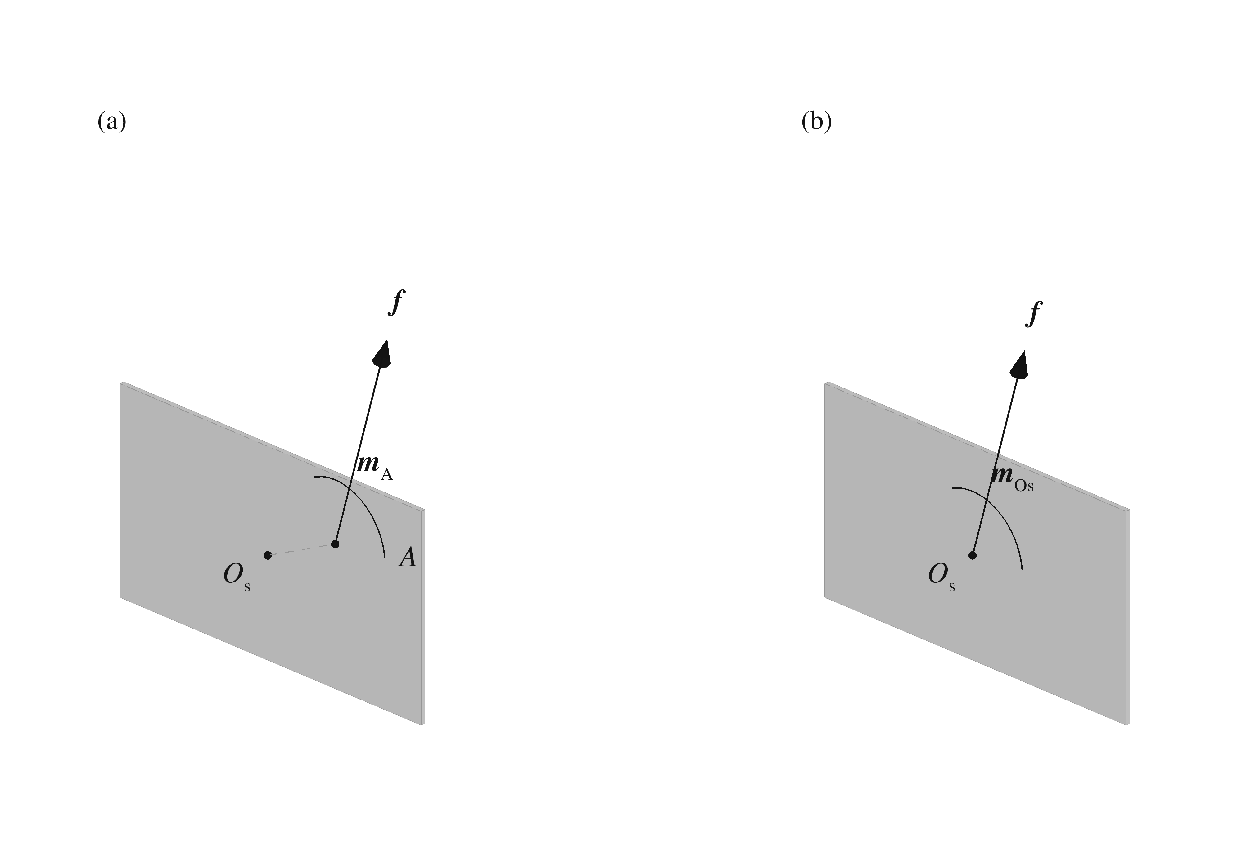
\includegraphics[width=.96\linewidth,height=.40\textheight,keepaspectratio]{figures/tecplot/concept_carga-seccion.pdf}
\caption[Transferencia de cargas aerodinámicas]{Transporte de una resultante de sección: (a) fuerza y momento aplicados en un punto $A$ y (b) representación equivalente respecto de $O_s$. La fuerza se conserva y el momento cambia según $\vct m_{O_s}=\vct m_A+\vct r_A\times\vct f$. Los arcos señalan la dirección de los momentos; sus radios son ilustrativos.}\label{fig:carga-seccion}
\end{figure}

Al linealizar, la variación aerodinámica se separa en
\begin{equation}
 \delta\vct f_a
 =\mathsf F_{a,q}\vct\eta+\mathsf F_{a,v}\dot{\vct\eta}
  +\delta\vct f_{a,\mathrm{imp}}(t).
\end{equation}
El último término corresponde a la variación impuesta del flujo; los dos primeros recogen la dependencia de la fuerza respecto del movimiento estructural. Sus contribuciones a la rigidez y al coeficiente de velocidad son $-\mathsf F_{a,q}$ y $-\mathsf F_{a,v}$. En particular, la dirección de una carga seguidora cambia con la orientación del componente. La derivada de esa dirección debe conservarse y puede producir una tangente no simétrica. La dependencia de la carga respecto del movimiento se evalúa con la misma ley utilizada para determinar el estado de operación.

\subsection{Excitación sísmica y recuperación del movimiento absoluto}
La traslación impuesta del terreno se denota $\vct u_B(t)$ y su aceleración $\vct a_B(t)=\ddot{\vct u}_B(t)$. Para construir la carga equivalente se parte de las coordenadas completas, incluidas las de apoyo, y se escribe
\begin{equation}
 \vct q_{\mathrm{abs}}=\mathsf T(t)\vct z+\mathsf\Gamma_f\vct u_B.
 \label{eq:movimiento-base}
\end{equation}
El vector $\vct z$ reúne las coordenadas independientes relativas y la matriz $\mathsf T$ impone la compatibilidad. La matriz $\mathsf\Gamma_f$ distribuye una traslación uniforme de la base: sus bloques traslacionales son identidades y sus bloques angulares son nulos cuando todas las componentes se expresan en ejes inerciales. Una descripción en ejes móviles requiere transformar también esta influencia y conservar sus derivadas.

Con $\mathsf\Gamma_f$ constante, la sustitución de \eqref{eq:movimiento-base} en las ecuaciones completas y la proyección sobre los movimientos admisibles producen la contribución
\begin{equation}
 \vct f_B=-\mathsf T^\tr\left(
 \mathsf M\mathsf\Gamma_f\ddot{\vct u}_B+
 \mathsf D\mathsf\Gamma_f\dot{\vct u}_B+
 \mathsf K\mathsf\Gamma_f\vct u_B\right).
 \label{eq:sismo-general}
\end{equation}
En esta ecuación, $\mathsf M,\mathsf D,\mathsf K$ son los coeficientes de las ecuaciones completas antes de eliminar los apoyos. Si las fuerzas elásticas y disipativas se definen respecto del movimiento relativo al terreno, o anulan la traslación rígida correspondiente, la expresión se reduce a
\begin{equation}
 \vct f_B=-\mathsf P_B\vct a_B,\qquad
 \mathsf P_B=\mathsf T^\tr\mathsf M\mathsf\Gamma_f.
 \label{eq:sismo-inercia}
\end{equation}
La matriz $\mathsf P_B$ conserva el acoplamiento de masa con las coordenadas prescritas. Una carga aerodinámica dependiente de la velocidad absoluta puede aportar términos adicionales asociados a $\dot{\vct u}_B$; estos se mantienen en la ley de carga.

La aceleración absoluta se reconstruye diferenciando la relación cinemática,
\begin{equation}
 \ddot{\vct q}_{\mathrm{abs}}
 =\mathsf T\ddot{\vct z}
  +2\dot{\mathsf T}\dot{\vct z}
  +\ddot{\mathsf T}\vct z
  +\mathsf\Gamma_f\vct a_B.
\end{equation}
Cuando $\vct q_{\mathrm{abs}}$ representa únicamente la perturbación, la aceleración total de una partícula se obtiene añadiendo la aceleración de su movimiento nominal. De esta forma se distinguen la aceleración relativa de vibración, la contribución sísmica y la aceleración asociada al giro.

\section{Frecuencias naturales y modos de vibración}
Para coeficientes constantes, las vibraciones libres de \eqref{eq:finaldynamic} se buscan como $\vct\eta=\vct\phi e^{\lambda t}$, lo que conduce al problema cuadrático \cite{tisseur}
\begin{equation}
 (\lambda^2\mathsf M_0+\lambda\mathsf D+\mathsf K)\vct\phi=\vct0.
\end{equation}
El autovector $\vct\phi$ describe una dirección de perturbación del estado $\vct q_0$; no determina por sí mismo ese equilibrio. Las matrices dependen de $\vct q_0$ y $\Omega$, por lo que cambiar el estado de operación cambia el problema modal. Cuando $\mathsf D=0$, $\mathsf M_0$ es positiva definida y $\mathsf K$ es simétrica, se recupera $\mathsf K\vct\phi_j=\omega_j^2\mathsf M_0\vct\phi_j$. En presencia de efectos giroscópicos, la formulación cuadrática es la forma general apropiada y los autovectores pueden ser complejos.

Existe una relación especial que conviene no confundir con lo anterior. En un problema estático lineal conservativo $\mathsf K\vct q_0=\vct f_0$, con $\mathsf K$ invertible y una base modal completa normalizada por masa, puede escribirse
\begin{equation}
 \vct q_0=\sum_j\vct\phi_j\frac{\vct\phi_j^{\tr}\vct f_0}{\omega_j^2},
 \qquad\vct\phi_i^{\tr}\mathsf M_0\vct\phi_j=\delta_{ij}.
\end{equation}
Es una expansión de una solución estática en una base, no una identidad entre equilibrio y modo. No se aplica directamente si hay modos rígidos de frecuencia cero, rigidez singular o un equilibrio no lineal dependiente de la deformación.

\section{Límite entre equilibrio relativo y régimen periódico}
Cuando las ecuaciones conservan una dependencia periódica del azimut, el estado de operación puede ser una trayectoria $\vct q_p(t)$ con período $2\pi/\Omega$ y no un vector constante. La perturbación se define entonces por $\vct q=\vct q_p+\vct\eta$ y satisface un sistema lineal de coeficientes periódicos. Su estabilidad se estudia mediante la evolución sobre un período, no interpretando sin más los autovalores de una matriz evaluada en un único azimut como frecuencias globales.

Una evaluación a azimut fijo es una aproximación local que debe identificarse como tal. Las transformaciones multípala pueden simplificar la periodicidad de un rotor simétrico \cite{bir}, pero no garantizan eliminarla bajo cargas o propiedades arbitrarias. Con esta separación quedan definidos los niveles del modelo: cinemática exacta de sección rígida, discretización estructural, estado de operación adoptado y dinámica lineal de sus perturbaciones. Cada nivel conserva sus hipótesis y su alcance sin atribuir al modelo lineal capacidades que pertenecen a una formulación no lineal o periódica más general.
\appendix
